\documentclass[
%% alle weiteren Papierformat einstellbar:
a4paper, %apaper,
%% keine Seitenzahlen:
%empty,
%% Schriftgröße (12pt, 11pt (Standard)):
11pt,
%% kleinere Überschriften:
%smallheadings,
%bibliography=totoc,
]
{scrartcl}

\input{packages.latex}

% chktex-file 18

\title{Network Security}
\subtitle{Zusammenfassung}
\author{Martin Darmüntzel}

\begin{document}

\maketitle

\tableofcontents

\pagebreak

\section{Motivation}%
\label{sec:motivation}

\begin{definition}[Netzwerk]
  Ein \emph{Netzwerk} ist eine Gruppe von Computern, die bekannte Kommunikationsprotokolle
  über digitale Verbindungen nutzen um Ressourcen zu teilen, die von den Netzwerkknoten
  bereitgestellt werden.

  Die Verbindungen zwischen den Knoten basieren auf physisch verkabelten, optischen, und
  kabellosen Methoden.
\end{definition}

\section{Building Blocks}%
\label{sec:building_blocks}

Folgende Komponenten stehen zur Verfügung:
\begin{itemize}
  \item Zonen, interne oder private Netzwerke, demilitarisierte Zonen
  \item Firewalls
  \item Intrusion Detection Systems, Intrusion Prevention Systems
  \item Proxies
  \item Virtual Private Networks
\end{itemize}

\subsection{Zonen - demilitarisierte Zone}%
\label{sub:zonen_dmz}

Eine DMZ ist ein kleines Netzwerk, das öffentlich verfügbare Dienste (wie HTTP) anbietet.
Sie wird oft von einer Firewall geschützt und befindet sich außerhalb des internen
Netzwerks.
Sie wird als weniger sicher als das interne Netzwerk angesehen.

\begin{figure}[h]
  \centering
  \subcaptionbox{mit einer Firewall}{
    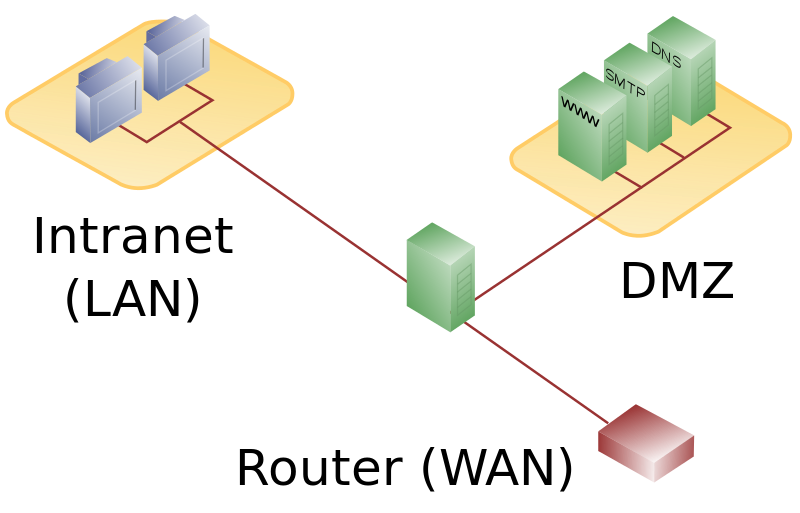
\includegraphics[width=0.4\linewidth]{bilder/dmz_1.png}
  }
  \subcaptionbox{mit zwei Firewalls}{
    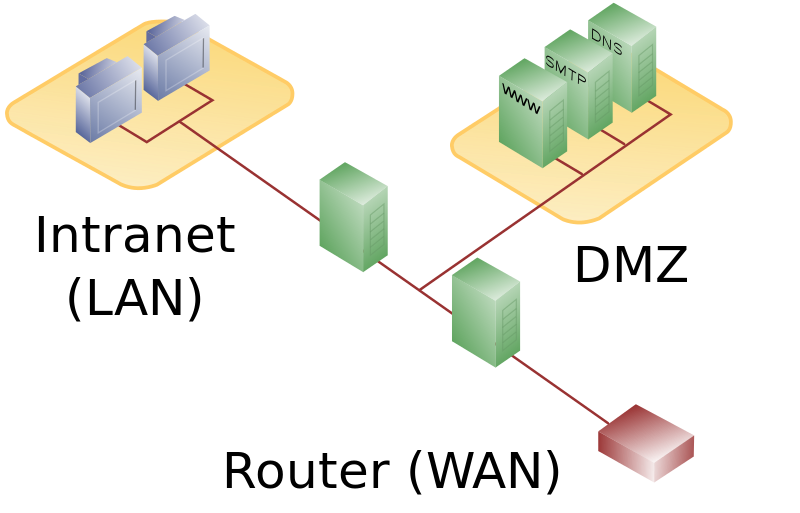
\includegraphics[width=0.4\linewidth]{bilder/dmz_2.png}
  }
  \caption{Netzwerk mit DMZ}
  \label{fig:dmz}
\end{figure}

\subsection{Internes Netzwerk}%
\label{sub:internes_netzwerk}

Schränkt den Zugang zum externen Netzwerk ein.
Der Zugang ist, wenn überhaupt, nur durch Gateways möglich.
Warum ist das nötig, wenn Angreifer sowieso nur im externen Internet sind?
Damit mögliche Schadsoftware nicht nach draußen kommunizieren kann.

Interne Angriffsrisiken hängen ab von:
\begin{itemize}
  \item Anzahl der Benutzer
  \item Vertrauen in die Nutzer
  \item Art und Weise wie die Benutzer auf das Netzwerk zugreifen
  \item Fähigkeiten der Benutzer
\end{itemize}

\subsection{Firewalls}%
\label{sub:firewalls}

Firewalls entscheiden ob Traffic passieren darf oder nicht.
Arten von Firewalls:
\begin{itemize}
  \item packet filter
  \item stateful firewalls
  \item proxy firewall
\end{itemize}

Offene Fragen bei Firewalls:
\begin{itemize}
  \item Woher kommen die Regeln?
  \item Wer entscheidet was erlaubt ist?
  \item Wer wartet die Firewall?
\end{itemize}

\subsection{Intrusion Detection Systems}%
\label{sub:intrusion_detection_systems}

Ein IDS erkennt Angriffe bzw. verdächtigen Traffic.
Es hilft dabei Firewalls aufzusetzen und zu konfigurieren.
Es ist normalerweise transparent für Benutzer und Angreifer.
Zwei wesentliche Prinzipien:
\begin{itemize}
  \item Mustererkennung
  \item Anomalieerkennung
\end{itemize}

Offene Fragen bei IDS:
\begin{itemize}
  \item Wie können Anomalien erkannt werden? Welche Klassifizierungsalgorithmen stehen zur
    Verfügung?
  \item Was macht man mit den gewonnenen Informationen?
  \item Welche Reaktionen können auf einen Alarm erfolgen?
\end{itemize}

\subsection{Proxies}%
\label{sub:proxies}

Teilen sehr stark das interne und externe Netzwerk.
Normalerweise auf dem application layer.
Verhindern, dass „bestimmte“ Informationen in das interne Netzwerk geschickt werden
(Viren, Pornos, illegale Informationen).
Verhindern, dass Informationen ins externe Netzwerk gesendet werden.
Wird oft mit anderen Systemen kombiniert (Virenfilter, Spamfilter, IDS).

Proxies sind selbst ein beliebtes Ziel für Angriffe.

\subsection{VPNs}%
\label{sub:vpns}

VPNs erzeugen einen gemeinsamen Adressbereich.
Sie schützen die Kommunikation über ein ungeschütztes Netzwerk.
Die Kommunikationspartner müssen sich gegenseitig authentifizieren.
VPNs bieten Kosteneinsparungen gegenüber festgeschalteten Verbindungen.

Offene Fragen zu VPNs:
\begin{itemize}
  \item Welche kryptographischen Verfahren werden genutzt?
  \item Wie werden Zugangstokens verwaltet?
  \item Welchen Einfluss haben VPNs auf Geschwindigkeit, Routing und andere
    Sicherheitskomponenten?
\end{itemize}

\section{Kryptographische Grundlagen}%
\label{sec:kryptographische_grundlagen}

Kerckhoffsche Annahme: Sicherheit hängt nur von den Schlüsseln ab und nicht vom Unwissen
des kryptographischen Verfahrens.

Grundlegendes Verfahren:
Der Klartext $p$ wird mittels Schlüssel $k$ durch die Verschlüsselungsfunktion $E$ zum
Geheimtext verschlüsselt:
\begin{align*}
  c = E_k(p)
\end{align*}
Dieser Geheimtext wird versendet und vom Empfänger mit der Entschlüsselungsfunktion $D$
und dem Schlüssel $k'$ entschlüsselt, sodass gilt:
\begin{align*}
  D_{k'}(c) = D_{k'}(E_k(p)) = p
\end{align*}
Der Angreifer möchte den Klartext herausfinden und braucht dazu den Schlüssel zum
Entschlüsseln (dies kann der gleiche Schlüssel sein wie zum Verschlüsseln).

Es gibt bspw. folgende Angriffsmodelle:
\begin{itemize}
  \item ciphertext-only
  \item known-plaintext
  \item (adaptive) chosen-plaintext
  \item (adaptive) chosen-ciphertext
\end{itemize}

\subsection{Symmetrische Verschlüsselung}%
\label{sub:symmetrische_verschlusselung}

Hierbei ist der Schlüssel zum Verschlüsseln der gleiche, wie zum Entschlüsseln.
Es gibt je nach Anwendungsfall zwei verschiedene Verfahren:
\begin{itemize}
  \item stream cipher: Stromverschlüsselung.
    Der fortlaufende Klartext wird mittels XOR mit einem Schlüsselstrom
    (normalerweise ein Pseudozufallszahlengenerator) verknüpft.
    Der Seed des Pseudozufallszahlengenerators ist der Schlüssel $k$.
  \item block cipher: Blockverschlüsselung.
    Verschlüsselt den Klartext blockweise mit dem Schlüssel.
    Dabei muss ein Block immer voll gefüllt sein, sodass manchmal Padding nötig ist.
\end{itemize}

Besonderes Verfahren: one-time pad.
Der Schlüsselstrom ist eine reine zufällige Bitfolge, die Absender und Empfänger vorher
kennen.
Der Schlüssel muss genauso lang wie der Klartext sein.
Der Schlüssel darf sich selbst nicht wiederholen.
Dies ist dann bedingungslos sicher.

Praktische Verfahren nutzen wesentlich kürzere Schlüssel.
Diese sind nicht mehr bedingungslos sicher, aber rechnerisch undurchführbar zu brechen.

Beispiel: DES (ist aber unsicher, weil die Schlüssellänge zu kurz ist).

\subsection{Asymmetrische Verschlüsselung}%
\label{sub:asymmetrische_verschlusselung}

Hierbei ist der Schlüssel zum Entschlüsseln $k$ verschieden zum Verschlüsselungsschlüssel
$k'$.
Es ist rechnerisch undurchführbar $k'$ aus $k$ zu ermitteln.
Daher kann $k$ öffentlich gemacht werden (public key).

\subsection{Hybride Verschlüsselung}%
\label{sub:hybride_verschlusselung}

Symmetrische Verschlüsselung ist schnell und asymmetrische Verschlüsselung ist langsam.
Bei symmetrischer Verschlüsselung muss jedoch der Schlüssel übertragen werden.
Lösung: nutze erst asymm. Verschlüsselung um eine Nachricht und Sessionkey zu übertragen
und danach symm. Verschlüsselung für die weitere Kommunikation.
Siehe~\ref{fig:Hybride_Verschlüsselung}.

\begin{figure}[h]
  \centering
  \includegraphics[width=0.9\linewidth]{bilder/Hybride_Verschlüsselung.png}
  \caption{Hybride Verschlüsselung}
  \label{fig:Hybride_Verschlüsselung}
\end{figure}

\subsection{Kryptographische Hashfunktionen}%
\label{sub:kryptographische_hashfunktionen}

Eine Hashfunktion $h$ macht aus einer Nachricht beliebiger Länge einen Hashwert mit fester
Länge.

Anforderungen:
\begin{itemize}
  \item Einweg: sei $y$ ein gegebener Hashwert, dann ist es rechnerisch undurchführbar
    eine Nachricht $x$ zu finden, sodass $h(x) = y$ gilt.
  \item schwacher Kollisionswiderstand: sei $x$ eine Nachricht, dann ist es rechnerisch
    undurchführbar eine andere Nachricht $x'$ zu finden, sodass $h(x) = h(x')$ gilt.
  \item (starker) Kollisionswiderstand: es ist rechnerisch undurchführbar zwei Nachrichten
    $x$ und $x'$ zu finden, sodass $h(x) = h(x')$ gilt.
\end{itemize}

Aufgrund des Geburtstagsparadoxons werden viele Bits gebraucht, damit Kollisionen
vermieden werden.
Sei $n$ die Anzahl der möglichen Hashwerte.
Dann kann eine Kollision bei $\sqrt{n}$ Nachrichten mit einer Wahrscheinlichkeit größer
als $0.5$ gefunden werden.
Bei einer Größe der Ausgabe von $h$ von $64$ Bits ist $\sqrt{n} = 232$ zu klein.
Die Größe der Ausgabe sollte mindestens $128$ oder besser $160$ sein.

Ein Problem bei Krypto im Netzwerk ist: die Nachrichten bzw. Pakete haben alle die gleiche
Struktur (z.\,B. Header, IP-Adressen, etc.) und enthalten damit teilweise bekannte
Klartexte.
Dadurch kann ein Angreifer möglicherweise Rückschlüsse auf den Schlüssel ziehen oder
verschlüsselte Blöcke durch eigene ersetzen.
Um das zu verhindern werden die verschlüsselten Blöcke miteinander durch \emph{cipher
block chaining} verbunden.

Hashfunktionen werden auch zum Signieren von Nachrichten verwendet (Nachricht hashen,
Hashwert verschlüsseln und anhängen).

Zum Schlüsselaustausch wird Diffie-Hellman verwendet:
\begin{enumerate}
  \item Alice und Bob einigen sich auf eine (große) Primzahl $p$ und $g < p$, wobei $g$
    ein Erzeuger von $\Integers_p$ ist.
    Auch Eve darf $p$ und $g$ kennen.
  \item Alice und Bob wählen zufällig eine Zahl $a$ bzw. $b$. aus $\{1, \ldots, p-1\}$
    aus, welche geheim bleiben.
  \item Alice berechnet ihren öffentlichen Schlüssel $A = g^a \mod p$ und sendet $A$ an
    Bob.
    Bob berechnet analog $B = g^b \mod p$ und sendet $B$ an Alice.
  \item Alice berechnet den gemeinsamen Schlüssel $K_1 = B^a \mod p$
    und Bob analog $K_2 = A^b \mod p$.

    Es gilt:
    \begin{align*}
      K_1 & = B^a \mod p = (g^b \mod p)^a \mod p = (g^b)^a \mod p = g^{ba} \mod p\\
      K_2 & = A^b \mod p = (g^a \mod p)^b \mod p = (g^a)^b \mod p = g^{ab} \mod p\\
      K_1 & = g^{ba} \mod p = g^{ab} \mod p = K_2
    \end{align*}
\end{enumerate}
Bei DH ist ein man in the middle Angriff möglich.

\subsection{Zertifikate}%
\label{sub:zertifikate}

Ein Zertifikat ist eine Datenstruktur bestehend aus:
\begin{itemize}
  \item dem öffentlichen Schlüssel
  \item Name des Besitzers des öffentlichen Schlüssels
  \item Name des Herausgebers
  \item Datum der Herausgabe
  \item Ablaufdatum
  \item mögliche andere Daten
  \item Signatur des Herausgebers
\end{itemize}

Zertifikate werden von einer Certification Authority (CA) herausgegeben, welcher vertraut
werden muss.
Zertifikate werden durch Certificate Directories verteilt, denen nicht vertraut werden
muss.
Eine Certificate Chain enthält Ketten von CAs und eigentlich muss man nur der Root-CA
vertrauen.

\section{Packet Filtering}%
\label{sec:packet_filtering}

\subsection{Funktionsweise}%
\label{sub:funktionsweise}

Netzwerkpakete werden je nach bestimmten Parametern akzeptiert oder zurückgewiesen,
z.\,B.:
\begin{itemize}
  \item Quelladresse, Quellport (falls das Protokoll das Konzept kennt)
  \item Zieladresse, Zielport (falls das Protokoll das Konzept kennt)
  \item Flags
\end{itemize}

Beispiel: TCP/IP
\begin{center}
  \begin{tabular}{cccccccc}
    \toprule
    \textbf{Layer} & \multicolumn{7}{c}{\textbf{Protokoll}}\\
    \midrule
    5-7 & Telnet & TFTP & FTP & SMTP & SNMP & DNS & \dots\\
    \midrule
    4 & \multicolumn{3}{c}{TCP} & \multicolumn{3}{c}{UDP}\\
    \midrule
    3 & IP & RARP & ARP & ICMP\\
    \midrule
    2 & \multicolumn{7}{c}{Logical Link Control \& Media Access Control}\\
    \midrule
    1 & \multicolumn{7}{c}{IEEE 802.2, Ethernet, ISDN, \dots}\\
    \bottomrule
  \end{tabular}
\end{center}

\begin{figure}[h]
  \centering
  \begin{subfigure}[c]{0.45\textwidth}
    \centering
    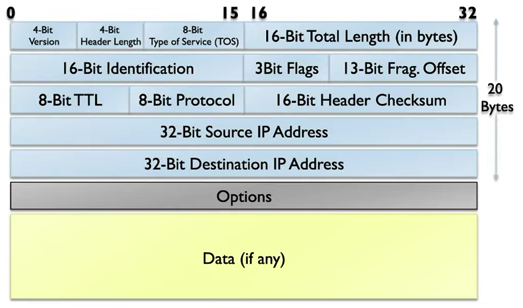
\includegraphics[width=1.0\textwidth]{bilder/ipv4_header.png}
    \subcaption{IPv4 Header}
    \label{fig:ipv4_header}
  \end{subfigure}
  \begin{subfigure}[c]{0.45\textwidth}
    \centering
    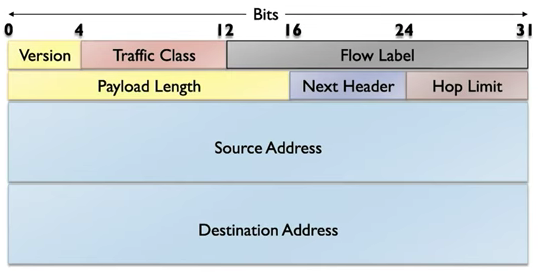
\includegraphics[width=1.0\textwidth]{bilder/ipv6_header.png}
    \subcaption{IPv6 Header}
    \label{fig:ipv6_header}
  \end{subfigure}

  \begin{subfigure}[c]{0.45\textwidth}
    \centering
    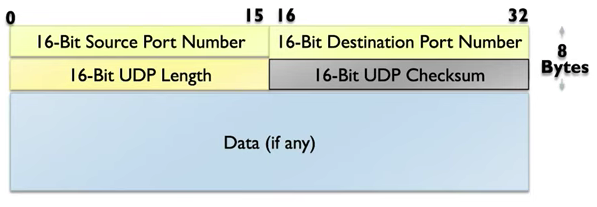
\includegraphics[width=1.0\linewidth]{bilder/udp_header.png}
    \subcaption{UDP Header}
    \label{fig:udp_header}
  \end{subfigure}
  \begin{subfigure}[c]{0.45\textwidth}
    \centering
    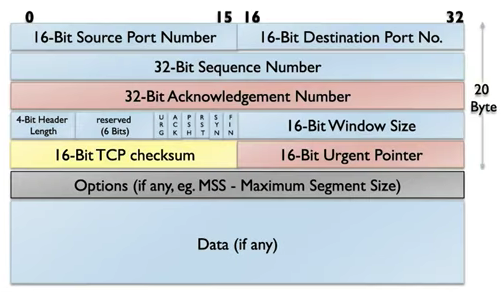
\includegraphics[width=1.0\linewidth]{bilder/tcp_header.png}
    \subcaption{TCP Header}
    \label{fig:tcp_header}
  \end{subfigure}
  \caption{Header von verschiedenen Protokollen}
\end{figure}

\paragraph{Regeln von Packet Filtern}%
\label{par:regeln_von_packet_filtern}

Die Regeln anhand von Flags, Adressen und Ports erstellt werden.
Man kann auch Pakete nach Inhalten filtern.

\paragraph{Arten von Regeln}%
\label{par:arten_von_regeln}

Erlaubende Regeln:
\begin{itemize}
  \item explizit bestimmten Zugang erlauben
  \item anderer Traffic wird normalerweise abgelehnt
\end{itemize}

Verbietende Regeln:
\begin{itemize}
  \item explizit bestimmte Pakete ablehnen
  \item anderer Traffic wird normalerweise zugelassen
\end{itemize}

Die Reihenfolge der Regeln ist wichtig.
Große Anzahl an Regeln ist meist verwirrend.
Best practice kann sein: verbiete alles außer anderweitig angegeben.
Beispiel:
\begin{itemize}
  \item \texttt{deny ip host 205.205.205.1 any}

    verbietet alle IP Pakete vom angegebenen Host

  \item \texttt{permit tcp host 205.205.205.1 any}

    erlaubt alle TCP Pakete vom angegebenen Host
\end{itemize}

Ingress filtering (Eingangskontrolle): filtert eingehende Pakete.
Verbietet Zugang von verdächtigen Quelladressen.

Egress filtering (Ausgangskontrolle): filtert ausgehenden Traffic.
Es dürfen nur Pakete das Netzwerk verlassen, deren Quelladresse im Netzwerk ist.
Falls Traffic von einem Knoten abgelehnt wird, dann ist das ein guter Kandidat für ein
Auditing.

Protokolle filtern: Dienste haben bestimmte Protokolle.
Daumenregel: erlaube nur Dienste, die wirklich benötigt werden.
Beispiele:
\begin{itemize}
  \item ICMP wird vollständig gefiltert
  \item UDP wird vollständig gefiltert
  \item TCP wird nur auf Port 80 erlaubt
  \item bei ICMP wird nur echo erlaubt
\end{itemize}

\paragraph{Probleme}%

Gefahr des Spoofings: externe Hosts können eine falsche Quelladresse vortäuschen und
weitere Authentifizierung ist nötig.
VPN wäre eine Lösung.

Routing: Pakete können Informationen zur Rückroute enthalten.
Die Routingtabelle könnte überschrieben werde.
Heutzutage aber kein Problem mehr.

Fragmentierung: Header eines Paketes könnte geteilt werden, sodass die Firewall nicht auf
den Header zugreifen kann.
Heutzutage auch kein Problem mehr.

Löcher: Chef möchte Sonderregelung, Angreifer nutzt das aus.

\subsection{Dynamisches Packet Filtering}%
\label{sub:dynamisches_packet_filtering}

Filterregel wird on-the-fly erstellt und gelöscht, nachdem die Verbindung geschlossen
wurde.
Der Filter beobachtet den ausgehenden Traffic und erstellt reflexive Regeln, aber nur
solange sie benötigt werden.
Beispiel: wenn eine ausgehende Verbindung zu 217.0.12.12:23 aufgebaut wird, dann wird eine
Regel erstellt, die eingehenden Traffic von 217.0.12.12:23 erlaubt.

\paragraph{Probleme}%
\label{par:probleme}

Regeln sind angreifbar indem falsche RST (reset) Pakete gesendet werden.
Ausgehender Traffic wird nicht gefiltert (Trojaner, Viren).

\section{Stateful Firewalls}%
\label{sec:stateful_firewalls}

\subsection{Funktionsweise}%
\label{sub:funktionsweise}

Stateful Firewalls \emph{kennen} den Zustand der Verbindungen und \emph{wissen} welche
Pakete in diesem Zustand erwartet werden.
Darauf können Regeln definiert werden, die nur in bestimmten Zuständen aktiv werden.
Stateful Firewalls arbeiten hauptsächlich auf dem transport layer (OSI Layer 4), aber auch
auf höheren Layern (OSI Layer $> 4$, wird dann \emph{stateful inspection}) genannt.
Zur Erinnerung: TCP ist Layer 4, HTTP arbeitet auf application layer (7).

\paragraph{Multi-layer inspection}%

Viele Protokolle basieren auf Protokollen einer geringeren Ebene.
Eine stateful Firewall kann mehrere Ebenen überwachen.

\paragraph{Neue Protokolle}%

Neue Protokolle müssen für die Konfiguration der Firewall beachtet werden.
Ein Beispiel sind Multimediaprotokolle, die viele Verbindungen zu externen Computern
herstellen, nachdem die initiale Verbindung hergestellt wurde.

\paragraph{Probleme}%
\label{par:probleme}

Hochperformante Firewalls brauchen manchmal geclusterte Hardware, aber stateful Firewalls
können nicht so einfach geclustert werden, da sie über einen gemeinsamen Zustand verfügen
müssen.

Wie können stateless Protokolle (UDP, DNS, ICMP, HTTP) von stateful Firewalls
gehandhabt werden?
Auch stateless Protokolle definieren, welche Pakete erwartet werden.
Mittels Timeouts können Pseudoverbindungen erzeugt werden.

\section{Proxy Firewalls}%
\label{sec:proxy_firewalls}

Bisher können wir nur einzelne Pakete filtern.
Wie können aber noch nicht die Inhalte der Verbindung filtern (z.\,B. Downloads).
Dafür braucht man Proxies.

Ein Proxy agiert für den internen Client und den externen Server.
Auf ihm laufen nur ein paar sichere und vertrauenswürdige Programme.
Ein Proxy kann die Inhalte der Verbindung bzw. der Pakete verändern, was zu ethischen
Problemen führen kann.

\subsection{Arten von Proxies}%
\label{sub:arten_von_proxies}

\paragraph{Forward Proxy}%
\label{par:forward_proxy}

Der Client befindet sich im internen Netzwerk und startet die Verbindung zum externen
Server.
Der Proxy nimmt die Verbindung entgegen und startet eine eigene Verbindung zum Server.

\paragraph{Reverse Proxy}%
\label{par:reverse_proxy}

Der Client befindet sich im externen Netzwerk und startet die Verbindung zum internen
Server.
Der Proxy nimmt die Verbindung entgegen und startet eine eigene Verbindung zum Server.
Wird benutzt um Dienste abzusichern, da jeder eingehende Traffic vom Proxy überwacht wird.

\subsection{Funktionsweise}%
\label{sub:funktionsweise}

Siehe \hyperref[sub:arten_von_proxies]{Arten von Proxies}.
Client und Server agieren niemals direkt miteinander.

Proxies können transparent oder intransparent sein.
Hier sind sie immer intransparent.
Die Clients müssen daher für Proxies konfiguriert werden, damit alles funktioniert.

Bei \emph{application level proxies} wird für jeden Dienst ein Proxy implementiert, sodass
nur bestimmter Traffic erlaubt ist, wie z.\,B.:
\begin{itemize}
  \item bestimmte Nutzer (wäre mit transparenten Firewalls unmöglich)
  \item bestimmte Adressen
  \item bestimmte Computer
\end{itemize}

Beispiel: \href{https://de.wikipedia.org/wiki/SOCKS}{SOCKS}

Da ein Proxy von Außen erreichbar ist, muss er gegen Angriffe abgehärtet sein.
Proxies sind normalerweise dual-homed (haben zwei Netzwerkschnittstellen).
Die interne Struktur des Netzwerks bleibt verborgen.
Auch passives Fingerprinting ist unmöglich (OS-Erkennung durch die Standardeinstellungen
bei Paketen wie z.\,B. \href{https://de.wikipedia.org/wiki/Time_to_Live}{TTL},
\href{https://de.wikipedia.org/wiki/TCP_Receive_Window}{TCP Receive Window Size},
TCP Optionen).
Ein \emph{bastion host} liefert nur die nötigsten Infos und bietet höchste Sicherheit.

\paragraph{Probleme}

Proxies haben Probleme mit verschlüsselten Verbindungen.
Wenn der Proxy Zugriff auf den Inhalt haben will, muss er diesen entschlüsseln, was aber
dank Ende-zu-Ende-Verschlüsselung unmöglich ist.

\paragraph{Vor- und Nachteile}%
\label{par:vor_und_nachteile}

Vorteile:
\begin{itemize}
  \item interne Struktur bleibt vor der externen Welt verborgen
  \item Traffic kann einfach überwacht werden
  \item nutzerbasierte Sicherheit ist möglich, Authentifizierung kann implementiert werden
  \item Spoofing wird verhindert, da der Proxy den ganzen Traffic der Außenwelt erzeugt
\end{itemize}

Nachteile:
\begin{itemize}
  \item Performance reduction
  \item Proxy ist ein single point of failure/attack
  \item application proxies müssen für jede Application entwickelt werden
  \item Software muss angepasst werden
  \item bastion host muss gehärtet werden
\end{itemize}

\section{Policies}%
\label{sec:policies}

Was ist eine Policy?
Eine Sicherheitspolicy definiert, was getan werden muss um auf Computern gespeicherte
Informationen zu schützen.
Sie definiert \emph{was} zu tun ist und \emph{wie} es evaluiert werden kann.
Wenn man nicht wahrnimmt, dass Policies missachtet werden, dann sind sie sinnlos.
Daher müssen sie evaluiert werden.
Eine Policy wird normalerweise aufgeschrieben.

Die Regeln einer Firewall repräsentieren eine Policy, sodass
\begin{itemize}
  \item alles verboten ist, außer es ist explizit erlaubt;
  \item alles erlaubt ist, außer es ist explizit verboten.
\end{itemize}
Die Wahrheit ist: alles ist verboten,
außer es ist explizit erlaubt oder es kommt trotzdem durch.

\subsection{Komplexität von Policies}%
\label{sub:komplexitat_von_policies}

Policies werden von Menschen definiert und befolgt.
Daher müssen sie verständlich sein.
Wenn sie zu komplex sind, dann sind sie nicht durchsetzbar.

Ein anderes Extrem ist jedoch: „Firmencomputer dürfen nicht für den persönlichen Gebrauch
genutzt werden!“
Diese Regel ist zu simpel und zu uneindeutig und daher nicht durchsetzbar.

Besser ist:
\begin{itemize}
  \item Sende keine Kettenbriefe.
  \item Sende keine Dateien.
  \item Nutze keine Pornoseiten.
\end{itemize}

\subsection{Entwicklung von Policies}%
\label{sub:entwicklung_von_policies}

Best practice:
\begin{enumerate}
  \item Risiken identifizieren
  \item Kommuniziere Funde
  \item erstelle oder aktualisiere Policies
  \item bestimme die Zustimmung der Policy mit den Mitarbeitern
  \item versuche eine \emph{Kultur} zu erschaffen
\end{enumerate}

\paragraph{Risiken identifizieren}%

Mach eine Sicherheitsanalyse: bestimme kritische Daten und Systeme und analysiere die
normale Nutzung des Netzwerks.
Schreib es auf.

\paragraph{Kommuniziere Funde}%

Berichte an’s Management: einfach, balanciert, kurz, zeige nicht auf einzelne Personen,
halte dich allgemein.

\paragraph{Erstelle oder aktualisiere Policies}%

Schreib sie auf und zwar spezifisch und klar.
Was muss gemacht werden?
Warum?
Wer ist verantwortlich?

Niemand liest mehr als 10 Seiten von Policies.
SMART: specific, measurable, achievable, realistic, time-based.

\paragraph{Bestimme die Zustimmung der Policy}%

Wenn eine Regel nicht messbar ist, dann ist sie nicht durchsetzbar.
Mögliche Inspektionen (audits): Stichproben, Analyse der Logfiles, Festplatten
durchsuchen.
Aber behalte den menschlichen Aspekt im Auge.
Niemand möchte gerne seine Browserhistory preisgeben.

\paragraph{Kulturelle Aspekte}%

Rede mit den Nutzern über die Risiken.
Erkläre die Policy bevor sie durchgesetzt wird.
Versuche „Anordnungen“ und authoritäres Verhalten zu vermeiden.

\section{Intrusion Detection Systems}%
\label{sec:intrusion_detection_systems}

IDS sind eine weitere Möglichkeiten um herauszufinden, was im Netzwerk abläuft.
Ein IDS verhindert keine Angriffe, aber erkennt Indizien für welche.

Ein IDS \emph{schüffelt} (sniffs) den Traffic, analysiert ihn und sucht nach Spuren für
\begin{itemize}
  \item Scans
  \item Aufklärungsaktivitäten
  \item Exploits
\end{itemize}
Dabei ist ein IDS voll transparent.

\subsection{Motivation}%
\label{sub:motivation}

Ohne ein IDS würden Admins Angriffe überhaupt nicht bemerken.
Folgende Infos werden gebraucht:
\begin{itemize}
  \item Welche Güter (assets) wurden angegriffen?
    Welcher Host wurde angreiffen?
    Server, Medien, User devices, Personen?
  \item Welche Daten wurden kompromittiert?
    Persönliche, medizinische, Logindaten, Zahlungen?
  \item Welche Methode wurde zum Angriff genutzt?
    Welcher Angriffsvektor wurde gewählt?
    Webseite, physisch, Backdoor?
\end{itemize}
Angriffe brauchen meist mehrere Einzelschritte, daher könnten Folgeschritte vermieden
werden.

\subsection{Anwendungen}%
\label{sub:anwendungen}

\begin{itemize}
  \item Betrugserkennung für Kreditkarten anhand der Zahlungsgeschichte.
  \item Einbruchserkennung durch Erkennung unnormalen Verhaltens.
\end{itemize}

\subsection{Typen}%
\label{sub:typen}

\paragraph{Netzwerkbasiert}%
\label{par:netzwerkbasiert}

Die Sensoren eines NIDS werden an bestimmten Punkten im Netzwerk (z.\,B. hinter der
Firewall) platziert und beobachten den Traffic von und zu allen Geräten.

\paragraph{Hostbasiert}%
\label{par:hostbasiert}

Ein HIDS läuft auf einzelnen Hosts/Geräten im Netzwerk und beobachten nur den Traffic des
Hosts.

\subsection{Methoden}%
\label{sub:methoden}

Um unnormalen Traffic zu erkennen werden z.\,B. \emph{statistische} Methoden benutzt.
Als Parameter nimmt man bspw: Ziel, Datenrate, Ports und Zeit.
Dann benutzt man Bayesianische Filter um die Wahrscheinlichkeit (likelihood) von Traffic
zu berechnen unnormal zu sein.
Diese Filter werden an normalem Traffic trainiert.

Eine andere Möglichkeit ist die Signaturerkennung.
Dabei werden Pakete nach bestimmten Mustern durchsucht.
Ein Beispiel: ein HTTP Request enthält
\begin{verbatim}
  get /scripts/..%c0%af../winnt/system32/cmd.exe?c+dir
\end{verbatim}
Dies wurde vom Nimda-Wurm benutzt um bestimmte Versionen von MS IIS zu exploiten.

Bei diesen Methoden kommt es immer zu falsch positiven und falsch negativen Warnung.
Wenn dies zu oft vorkommt, entsteht eine gewisse Ignoranz bei den Administratoren.
Daher müssen solche Regeln stetig verfeinert werden.

\section{Data Driven Security}%
\label{sec:data_driven_security}

Durch Datenanalyse kann das Risiko eines einzelnen Pakets ermittelt werden.
Mit der Zeit wurden viele Modelle und Ansätze entwickelt um Außenseiter zu erkennen.

\subsection{Problem}%
\label{sub:problem}

Die \emph{guten} Daten sollen von den \emph{schlechten} Daten unterschieden werden.
Weiterhin sollen die am besten passenden Charakteristika und Prozeduren gefunden werden,
die unser Problem lösen und uns helfen das System besser zu verstehen.

\begin{figure}[h]
  \centering
  \begin{subfigure}[c]{0.45\textwidth}
    \centering
    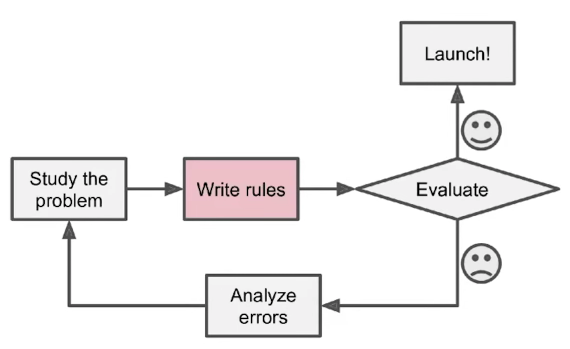
\includegraphics[width=0.95\linewidth]{bilder/without_ml.png}
    \subcaption{ohne Machine Learning}
    \label{fig:without_ml}
  \end{subfigure}
  \begin{subfigure}[c]{0.45\textwidth}
    \centering
    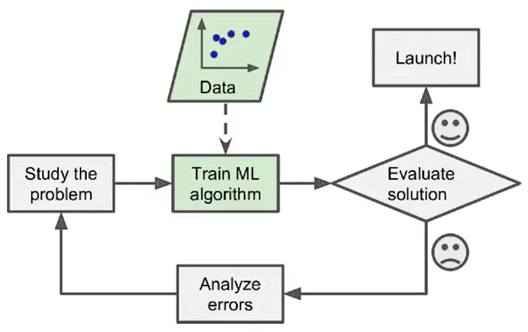
\includegraphics[width=0.95\linewidth]{bilder/with_ml.png}
    \subcaption{mit Machine Learning}
    \label{fig:with_ml}
  \end{subfigure}
  \caption{Problemlösen}
\end{figure}

Um das Problem besser zu verstehen, kann auch ML genutzt werden:
\begin{figure}[h]
  \centering
  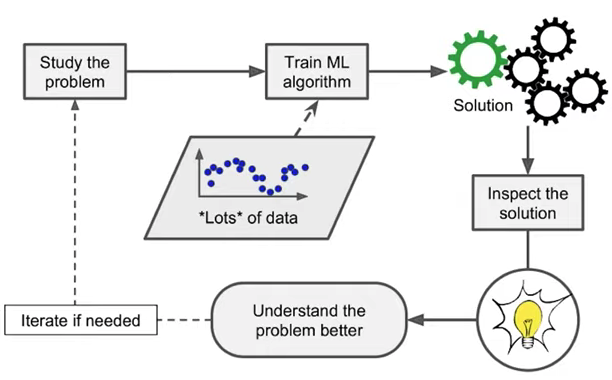
\includegraphics[width=0.6\linewidth]{bilder/human_learning_with_ml.png}
  \caption{Menschliches Lernen mit Hilfe von ML}
  \label{fig:human_learning_with_ml}
\end{figure}

\subsection{Lernen von Daten}%
\label{sub:lernen_von_daten}

\begin{description}
  \item[Domänenexpertise] um unser Fachwissen zu vergrößern
  \item[Datenmanagement] die Daten vorbereiten, speichern und warten
  \item[Programmierung] um Daten mit Analysen zu verbinden
  \item[Statistiken] um von den Daten zu lernen
  \item[Visualisierung] um die Ergebnisse effektiv zu kommunizieren
\end{description}

\subsection{Klassifizierung von ML Systemen}%
\label{sub:klassifizierung_von_ml_systemen}

Es gibt verschiedene Kategorien:
\begin{itemize}
  \item ob sie unter menschlicher Aufsicht trainiert werden
    (supervised, unsupervised, semi-supervised, reinforcement learning)
  \item ob sie inkrementell on the fly lernen können (online vs. batch learning)
  \item ob sie einfach nur neue Daten mit bekannten Daten vergleichen
    oder Muster erkennen und daraus wie Wissenschaftler ein Vorhersagemodell erzeugen
    (instance based vs. model-based learning)
\end{itemize}

\subsubsection{Supervised Learning}%
\label{ssub:supervised_learning}

Hier gibt’s Trainingsdaten mit Labels, mit der der Algorithmus gefüttert wird.
Dann wird der Algorithmus mit Testdaten getestet, bei denen die Labels fehlen.
Beispiele: Spamerkennung, Vorhersage von Werten mittels Regression.

Ein Parameter mit Wert der Daten wird \emph{Attribut} oder \emph{Feature} genannt.
Beispiel: ein gesetztes Flag in einem TCP-Paket.

\paragraph{Klassifikation}%
\label{par:klassifikation}

Heißt die Aufteilung in Klassen.
Trainiert wird mit Daten, deren Klasse bekannt ist und ein Label hat.

\paragraph{Regression}%
\label{par:regression}

Die Aufgabe hierbei ist einen numerischen Zielwert vorherzusagen, bspw. die Gefahr eines
IP-Pakets, anhand einer Menge von Features.
Das nennt man \emph{Prädiktor}.

\paragraph{Beste bekannte Algorithmen}%
\label{par:beste_bekannte_algorithmen}

\begin{itemize}
  \item $k$-nearest Neighbours
  \item Regression
  \item Support Vector Machines
  \item Decision trees and random forests
  \item Neurale Netzwerke
\end{itemize}

\subsubsection{Unsupervised learning}%
\label{ssub:unsupervised_learning}

Daten sind nicht gelabelt.
Aber die Daten können geclustert werden, also nach Ähnlichkeit gruppiert werden.

\paragraph{Typische Algorithmen}%
\label{par:typische_algorithmen}

\begin{itemize}
  \item Clustering (K-Means, DBSCAN, Hierarchical Cluster Analysis)
  \item Anomalieerkennung und novelty detection (one-class SVM, Isolation Forest)
  \item Visualisierung und Dimensionsreduktion (Principal Component Analysis PCA, Kernel
    PCA, \ldots)
  \item Association rule learning (Apriori, Eclat)
\end{itemize}

\subsubsection{Semisupervised learning}%
\label{ssub:semisupervised_learning}

Hier haben nicht alle Daten ein Label, weil die Datenmarkierung aufwändig ist.
Es soll aber immer noch zwischen guten und schlechten Daten unterschieden werden.

\subsubsection{Reinforcement learning}%
\label{ssub:reinforcement_learning}

Das lernende System, der Agent, kann die Umwelt beobachten, Aktionen wählen und
durchführen, und dafür Belohnungen oder Bestrafungen erhalten.
Es muss dann für sich selbst lernen, eine sog. Policy bestimmen, die die größte Belohnung
über die Zeit liefert.
Eine Policy definiert, welche Aktion in welcher Situation durchgeführt werden soll.

\subsection{Beispiele}%
\label{sub:beispiele}

Datenquellen für intrusion detection:
\begin{itemize}
  \item Pakete pro Sekunde
  \item Pakete pro Sekunde pro Tageszeit
  \item Requests pro Zeit
  \item Requests pro Zeit und Port
  \item Anzahl verschiedener Quelladressen pro Zeit
  \item Ort der Quelladressen
\end{itemize}

Infizierte Knoten:
\begin{itemize}
  \item Auslastung der Prozesse und des Speichers wird gemessen
    und mittels SVM in infizierte und saubere Knoten unterteilt
\end{itemize}

Visualisierung:
\begin{itemize}
  \item Geolocation
  \item Verteilung von IP-Adressen
  \item Verteilung der Infektionen in den Adressblöcken
  \item Traffic über die Zeit
  \item Verteilung der Ports
  \item Matrix von Angriffsvektor und Zielen
\end{itemize}

\subsection{Labeling vs. Scoring}%
\label{sub:labeling_vs_scoring}

Manchmal ist es schwierig ein binäres Label (normal, Außenseiter) für die Daten bzw.
Pakete zu vergeben.
Dann ist ein kontinuierlicher Score besser geeignet.
Wenn der Score irgendwann eine Schwelle überschreitet, dann wird Alarm geschlagen.

\subsection{Modellbasierte Ansätze}%
\label{sub:modellbasierte_ansatze}

Hier wenden wir ein Modell an, das normale Datenpunkte repräsentiert und Außenseiter sind
Punkte, die nicht ins Modell passen.
Dabei nehmen wir bspw. probabilistische Tests die auf statistischen Methoden basieren:
\begin{itemize}
  \item tiefenbasierte Ansätze: konvexe Hüllen werden um die Daten erzeugt, je weiter weg
    von der Mitte umso gefährlicher
  \item abweichungsbasierte Ansätze
\end{itemize}

\section{Honeypots, Tarpits und Proof of Work}%
\label{sec:honeypots_tarpits_und_proof_of_work}

\subsection{Honeypots}%
\label{sub:honeypots}

\begin{definition}
  Ein \emph{Honeypot} ist ein Sicherheitsmechanismus, der unauthorisierte Nutzungsversuche
  von Informationssystemen erkennen, ablenken und in gewisser Weise entgegenwirken soll.
\end{definition}

Im Unterschied zu einem IDS ist ein Honeypot aktiv, während ein IDS passiv ist.

Es gibt Honeypots aus Forschungszwecken bspw. für Anti-Viren-Software, der über neue Viren
und Varianten lernen will.
Netzwerkadmins wollen Informationen über aktuelle Bedrohungen sammeln und nutzen
normalerweise ein großes verteiltes Netzwerk von Fallen (auch als \emph{Honeynet}
bekannt).
Im produktiven Einsatz sollen Honeypots die Aufmerksamkeit von gut bekannten Angriffen auf
sich lenken und vom eigentlich Ziel ablenken.
Das ist nicht wirklich eine akzeptable Methode aus der Sicherheitsperspektive, aber es
hilft.

\paragraph{Wirkprinzipien}%
\label{par:wirkprinzipien}

Honeypots verhalten sich wie ein richtiges System.
Einem Angreifer sollte nicht auffallen, dass er mit einem Honeypot interagiert.
Sie zeichnen alle Nutzeraktionen auf, sodass Admins diese Spuren genau verfolgen können.
Danach analyieren Admins diese Angriffsmuster.

Honeynets beobachten nur die Netzwerkaktivitäten.

Spam traps sind veröffentlichte E-Mail-Adressen, die nur Spam anziehen sollen.
Die Trainingsdaten können später zur Spamerkennung genutzt werden.

Virus traps beobachten alle Virenaktivitäten in einer sand box.

Ein tarpit ist wie ein Honeypot, nur dass aktive Funktionen besitzt.
Er verlangsamt Angreifer, indem künstliche Wartezeiten in Protokollen eingebaut werden.
Damit werden die Kosten von Angriffen erhöht.

\paragraph{Proof of Work}%
\label{par:proof_of_work}

Ein POW-System fügt jedem Dienst einen gewissen Preis hinzu.
Dies kann bspw. CPU-Zeit für die Lösung eines Problems sein, welches sogar praktischen
Nutzen haben könnte.
Die Lösung des Problem muss aber schnell überprüfbar sein.

Beispiel: Wurzel modulo $p$.
Wähle eine Primzahl $p$ mit vernünftiger Größe (bspw. $1024$ bits).
Die Aufgabe besteht daraus zu einem gegebenen $x$ eine Zahl $y$ zu finden mit
$y^2 \equiv x \mod p$.
Sei bspw. $p=97$ und $x=50$, dann ist $y=27$.

Das kostet natürlich Energie, aber dämmt Spam ein.
Lohnt sich das?
Energie ist dabei die Währung.

Mit Application Specific Integrated Circuits (ASICs) können solche schwierigen Probleme
schneller gelöst werden.
Das führt zu einem Katz-und-Maus-Spiel.

Diese Arbeit kann für andere Angriffe benutzt werden (bspw. können CAPTCHAs ausgenutzt
werden).

\section{Public Key Infrastructure}%
\label{sec:public_key_infrastructure}

Wofür brauchen wir sowas?
Um Schlüssel zu signieren (Zertifikate erstellen), zu verteilen und falls nötig
zurückzuziehen.
Dies ist nötig um Man-in-the-middle Angriffe zu vereiteln.

Eine PKI erzeugt, verteilt und erklärt Zertifikate für ungültig.
Sie unterstützt die sichere Kommunikation und die Handhabung von rechtlich bindenen
Dokumenten (Signaturen, Unleugbarkeit).
Es liefert Dienste für sichere Zeitstempel.
Weiterhin kann es beim Privilegienmanagement helfen bzgl. der Authorisierung (nicht
Authentifizierung!).
Sie kann auch Teil von einem Digital Rights Management Systems sein.

Das Wesen von Public Key Krypto ist, dass ein Schlüssel zum Verschlüsseln und ein anderer
Schlüssel zum Entschlüsseln benutzt wird.
Der öffentliche Schlüssel muss dabei authentifiziert werden, damit nachgewiesen ist, dass
auch wirklich die Person dahintersteckt, die sie vorgibt zu sein.
Eine Certificate Authority (CA) übernimmt dabei diesen Signierungsprozess.

\subsection{Certificate Revocation}%
\label{sub:certificate_revocation}

Was passiert, wenn private Schlüssel verloren gehen oder gestohlen werden?
Verlorene private Schlüssel können nicht wiederhergestellt werden.
Gestohlene private Schlüssel sind ein Sicherheitsrisiko.

Also müssen neue Schlüssel erzeugt und die alten widerrufen werden (revoke).
Die Kommunikationspartner müssen dabei informiert werden, dass die widerrufenen Schlüssel
nicht mehr benutzt werden.
Dafür bietet eine PKI eine Liste von widerrufenen Schlüsseln: die Certificate Revocation
List (CRL).
Beispiel: \url{http://crl.verisign.com/Class3InternationalServer.crl}

\subsection{Certificate Distribution}%
\label{sub:certificate_distribution}

Wie kommen die Kommunikationspartner an die jeweiligen Schlüssel des anderen?
Sie können sich z.\,B. die Schlüssel einfach gegenseitig schicken.
Das funktioniert, weil die CA die Gültigkeit der Schlüssel gewährleistet.
Die Schlüssel können aber auch über eine Certificate Management Facility verwaltet werden,
sodass sich die Partner die Schlüssel problemlos herunterladen können.

Dafür wird normalerweise X.509 und LDAP genutzt.
X.509 wird dabei genutzt, um die Interoperabilität zwischen verschiedenen Anwendungen zu
gewährleisten (Webserver, E-Mail, VPN-Gateways).
Ein X.509 Zertifikat enthält dabei bspw. folgende Informationen:
\begin{itemize}
  \item Version
  \item Seriennummer
  \item Signatur
  \item ausstellende CA
  \item ID der ausstellenden CA
  \item Gültigkeitsdauer
  \item Inhaber
  \item Schlüsselinformationen des Inhabers: Public-Key-Algorithmus, Public-Key des
    Inhabers
  \item genutzter Signaturalgorithmus
  \item Signatur
\end{itemize}

Andere Formate: Public Key Cryptography Standards (PKCS).

\section{Hardware Security Modules}%
\label{sec:hardware_security_modules}

Für eine CA müssen die privaten Schlüssel sicher gelagert werden.
Nur die richtigen Personen dürfen auf die Schlüssel zugreifen.
Die Schlüssel dürfen nicht verändert werden und müssen gegen Diebstahl und Verlust
geschützt werden.
Dabei reicht es nicht aus, die Schlüssel als normale Datei auf einer Festplatte zu
speichern, da dies bestimmte Angriffe erlaubt.

\subsection{Speicherung eines Schlüssels}%
\label{sub:speicherung_eines_schlussels}

Schlüssel können entweder eingegeben werden, wenn das Gerät gestartet wurde, oder sie
können in einem Festspeicher (HDDs, SSDs, ROMs, Silikonstrukturen, RAM) gespeichert
werden.
Wenn sie aber irgendwo abgespeichert werden, sind sie anfällig für Lauschangriffe
(\emph{eavesdropping)}.

Dafür gibt’s jetzt spezielle Module: Hardware Security Module.
Ein HSM ist ein physikalisches Rechengerät (physical computing device),
das digitale Schlüssel verwaltet und schützt,
Verschlüsselungs- und Entschlüsselungsfunktionen für digitale Signaturen,
starke Authentifizierung und andere kryptographische Funktionen ausführt.
Das sind normalerweise Einsteckkarten oder externe Geräte, die man an einen Rechner oder
einen Netzwerkserver anschließt.
Ein HSM enthält einen oder mehrere sichere Kryptoprozessorchips.
Man kann einen Schlüssel auf dem HSM erzeugen, aber es gibt keine Funktionen, um die
Schlüssel zu extrahieren.
Einfaches Beispiel: eine Kreditkarte mit NFC.

\subsection{Funktionen eines HSM}%
\label{sub:funktionen_eines_hsm}

Sie erzeugen onboard kryptographische Schlüssel.
Dafür sind viele Zufallszahlen nötig und richtige Zufallszahlen sind auf einem
deterministischem Computer schwierig zu erzeugen.
Sie speichern die Schlüssel sicher ab – zumindest die sensitivsten Schlüssel (master
keys).
Sie führen die Verschlüsselung oder digitale Signierung aus.

Wichtig ist dabei: achte auf Seitenkanalangriffe!

\subsection{Backup eines Schlüssels}%
\label{sub:backup_eines_schlussels}

Dabei gibt es zwei Methoden:
die \emph{multiple custodians method}
und die \emph{single custodian method}.

\paragraph{multiple custodians}%
\label{par:multiple_custodians}

Der Schlüssel wird in Teile gespalten und auf mehrere Verwahrer (custodians) verteilt.
Die Teile werden von einem zweiten zufällig gewählten Schlüssel (wrapping key)
verschlüsselt (verpackt).
Zur Wiederherstellung werden entweder beim Standardverfahren alle Verwahrer
oder bei einem $N$ aus $M$ Schema ein bestimmtes Minimum der Verwahrer benötigt.

\paragraph{single custodian}%
\label{par:single_custodian}

Hierbei wird der Schlüssel von einem speziell ausgewählten Schlüssel (wrapping key)
verschlüsselt.

\section{Enterprise Authentication}%
\label{sec:enterprise_authentication}

\begin{definition}
  \emph{Authentifizierung} ist der Prozess die Identität oder eine Eigenschaft (claim)
  von einer Entität (bspw. einer Person) nachzuweisen.
\end{definition}

\subsection{Prinzipien}%
\label{sub:prinzipien}

\begin{description}
  \item[wissensbasiert] PIN, Passwort, persönliche Informationen
  \item[besitzbasiert] SmartCard / SIM Karte, Kreditkarte, Schlüssel, RFID Token, Telefon,
    PC, DRM Modul
  \item[biometrisch] Retina, Iris, Fingerabdruck, DNA, Stimme, Unterschrift
\end{description}
Die Sicherheit wird durch Zwei-Faktor-Authentifizierung weiter verbessert, indem zwei
Methoden kombiniert werden.

Probleme der einzelnen Prinzipien:
\begin{description}
  \item[wissensbasiert] die Nutzer wählen ein schwaches Passwort,
    Nutzer vergessen die Passwörter, Passwort wurde anderweitig kompromittiert
  \item[besitzbasiert] Nutzer verlieren Token, Token wird kopiert
  \item[biometrisch] bestimmte biometrische Eigenschaften können kopiert werden,
    hat ethische Probleme (DNA liefert Aufschlüsse über Gesundheitszustand),
    schwierig zu handhaben
\end{description}

\subsection{Implementierungen}%
\label{sub:implementierungen}

\subsubsection{Kerberos}

Hier wird Authentifizierung und Authorisierung und der eigentliche Dienst voneinander
getrennt.


\subsubsection{RADIUS}

\section{Virtual Private Networks}%
\label{sec:virtual_private_networks}

Warum VPN?
\begin{itemize}
  \item Confidentiality (Vertraulichkeit)
  \item Authenticity
  \item Integrity
\end{itemize}
Überhaupt braucht man VPNs um eine sichere Verbindung über ein unsicheres Netzwerk
herzustellen.

\subsection{Funktionen}%

Ein VPN verbindet mind. zwei Endpunkte oder mehrere Netzwerke miteinander und erzeugt
damit einen gemeinsamen Adressbereich.
Das wird kombiniert mit Verschlüsselung und Authentifizierung.

Es gibt zwei Hauptarten von VPNs:
\begin{itemize}
  \item Host-to-Gateway VPN: für Remoteuser von Unternehmensressourcen
  \item Gateway-to-Gateway VPN: um einen verschlüsselten Tunnel zwischen zwei Gateways zu
    erzeugen
\end{itemize}

\subsection{Implementierungen}%

\begin{itemize}
  \item L2TP: Layer 2 Tunneling Protocol
  \item IPSec
\end{itemize}

\section{Multi factor Authentication}%
\label{sec:multi_factor_authentication}

\begin{itemize}
  \item offline tokens: brauchen ein vorher vereinbartes gemeinsames Geheimnis
    \begin{itemize}
      \item HOTP: HMAC-based One-time Password Algorithm, nutzt Counter
      \item TOTP: Time-based One-time Password Algorithm, nutzt aktuellen Zeitstempel
    \end{itemize}
  \item online tokens
    \begin{itemize}
      \item Universal 2nd Factor tokens mit Universal Authentication Framework; von der
        FIDO Alliance entwickelt und vorangetrieben
    \end{itemize}
\end{itemize}

\section{Digitale Forensik}%
\label{sec:digitale_forensik}



\section{Software und Firmware Bewertung}%
\label{sec:software_und_firmware_bewertung}




\pagebreak

\listoftodos

\end{document} % chktex 17
